% Created by tikzDevice version 0.6.2-92-0ad2792 on 2013-03-31 12:28:06
% !TEX encoding = UTF-8 Unicode
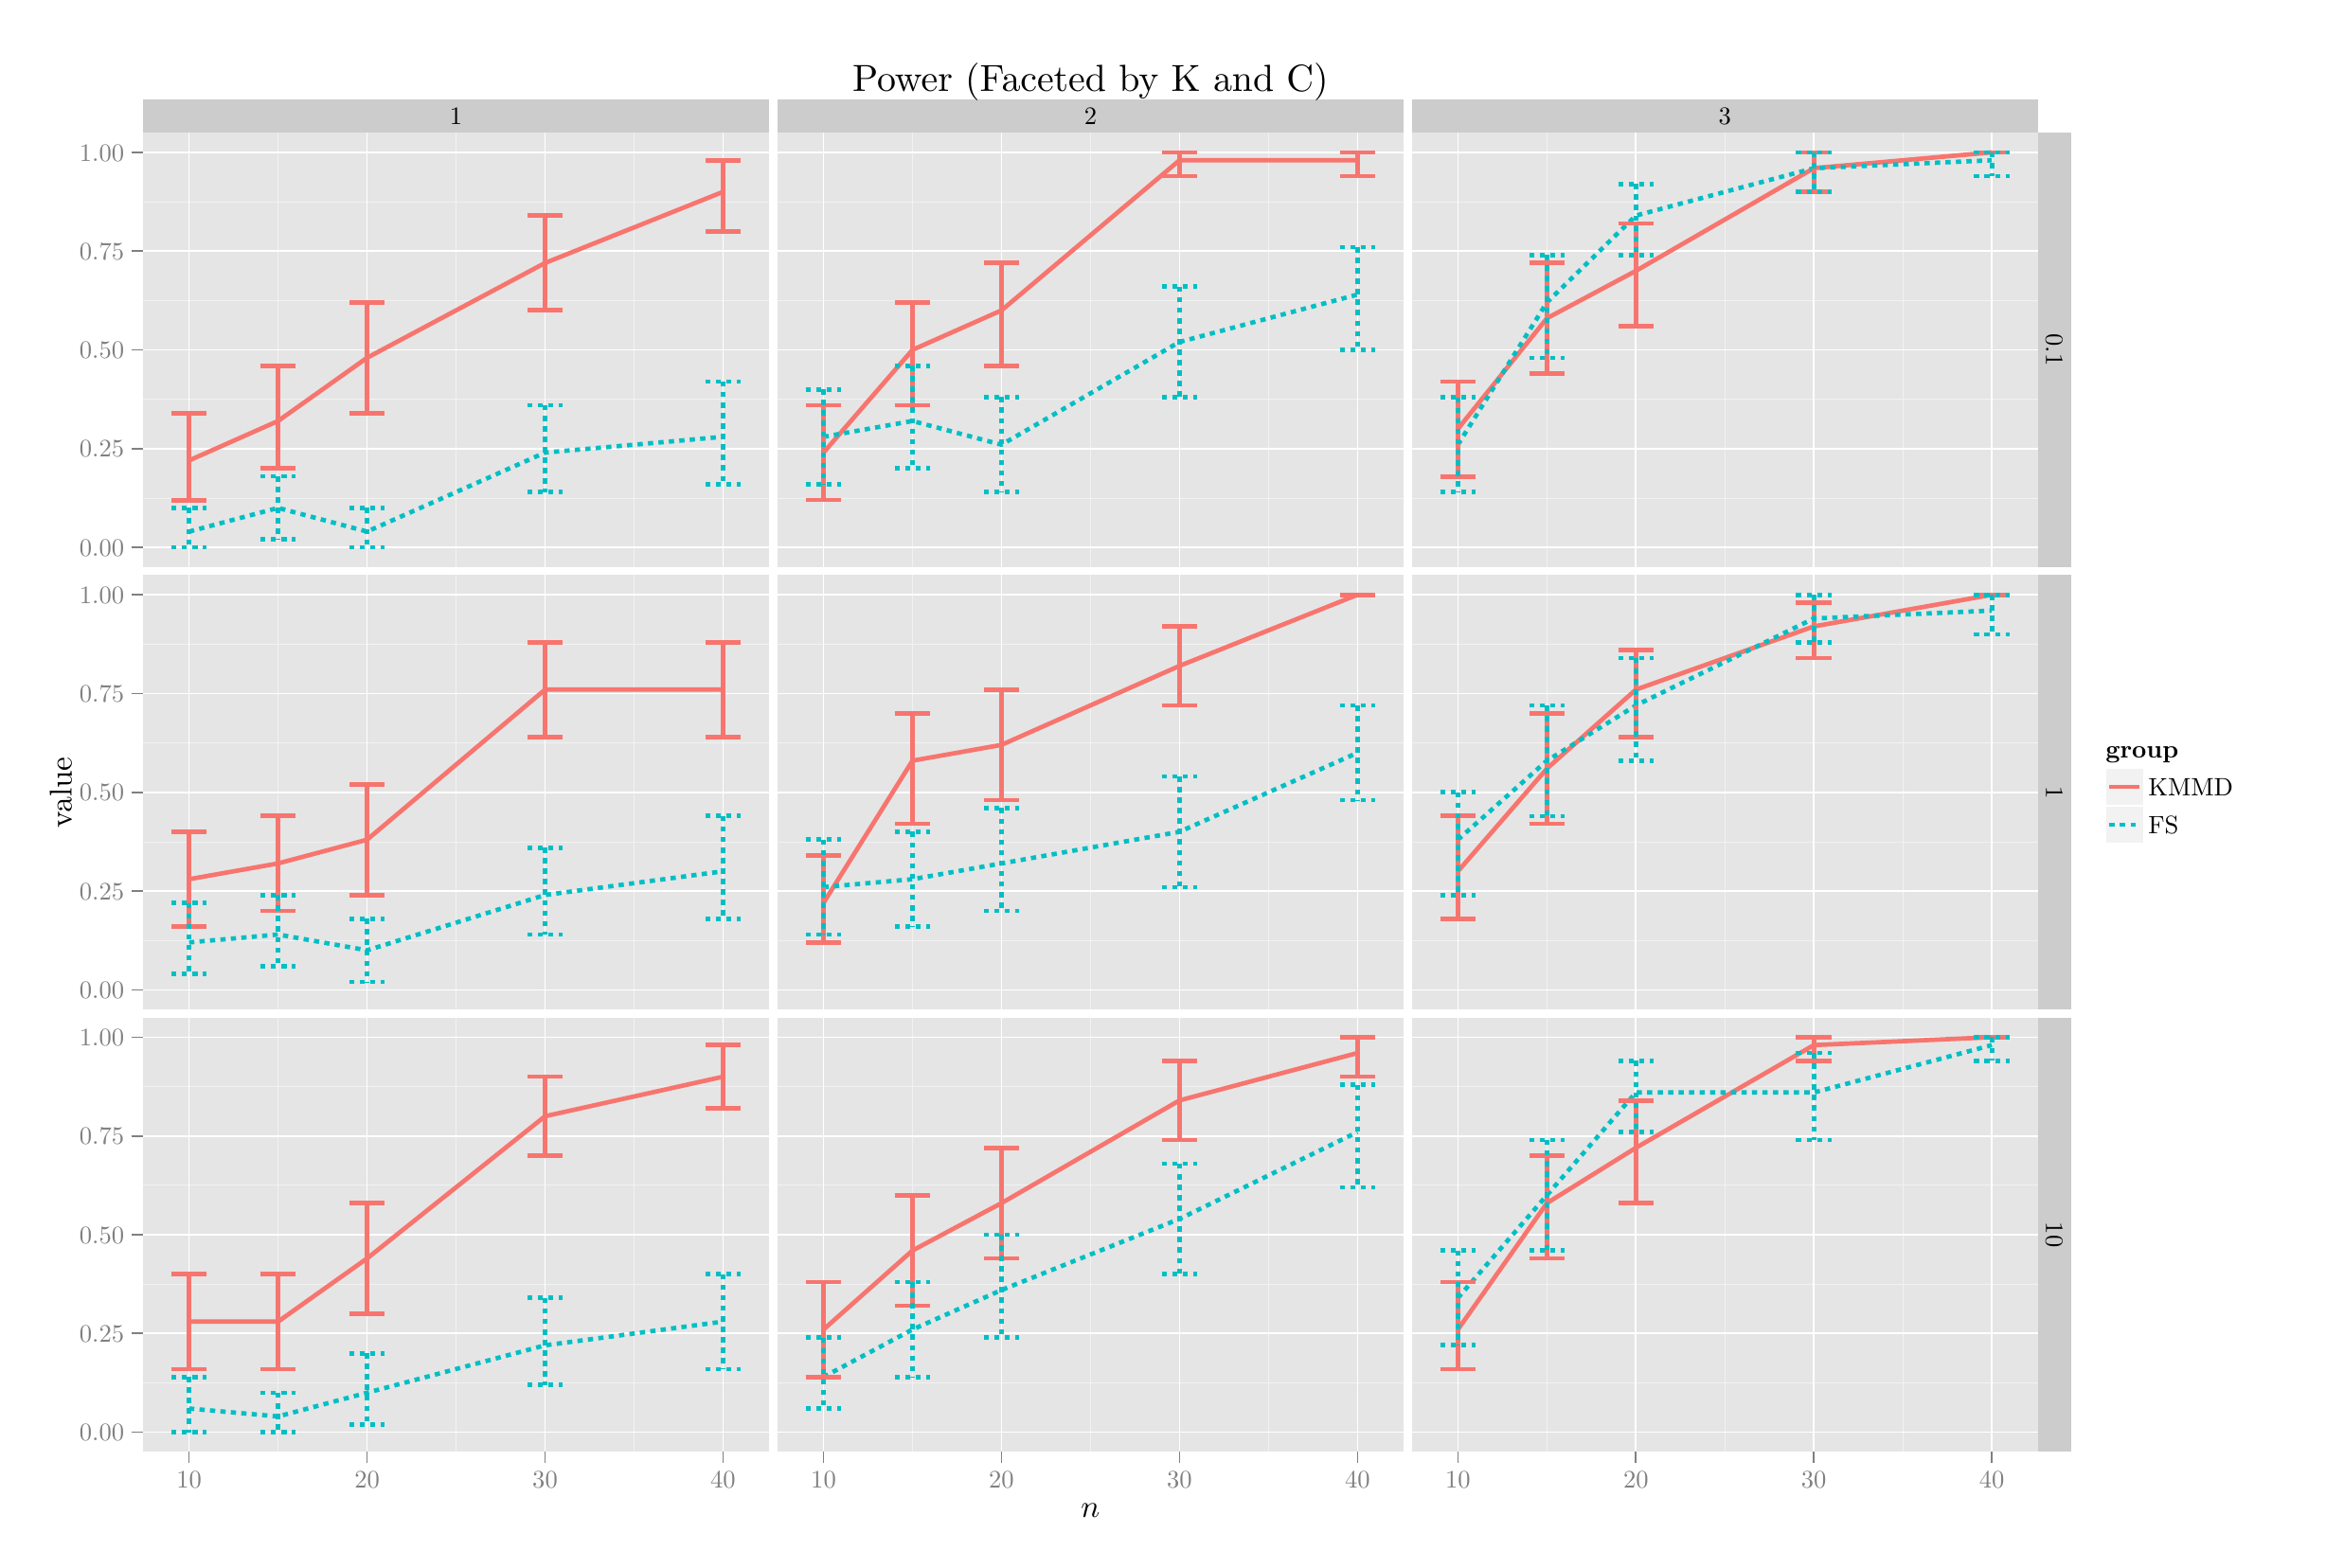
\begin{tikzpicture}[x=1pt,y=1pt]
\definecolor[named]{fillColor}{rgb}{1.00,1.00,1.00}
\path[use as bounding box,fill=fillColor,fill opacity=0.00] (0,0) rectangle (867.24,578.16);
\begin{scope}
\path[clip] (  0.00,  0.00) rectangle (867.24,578.16);
\definecolor[named]{drawColor}{rgb}{1.00,1.00,1.00}
\definecolor[named]{fillColor}{rgb}{1.00,1.00,1.00}

\path[draw=drawColor,line width= 0.6pt,line join=round,line cap=round,fill=fillColor] (  0.00, -0.00) rectangle (867.24,578.16);
\end{scope}
\begin{scope}
\path[clip] ( 44.49,537.54) rectangle (283.53,550.17);
\definecolor[named]{fillColor}{rgb}{0.80,0.80,0.80}

\path[fill=fillColor] ( 44.49,537.54) rectangle (283.53,550.17);
\definecolor[named]{drawColor}{rgb}{0.00,0.00,0.00}

\node[text=drawColor,anchor=base,inner sep=0pt, outer sep=0pt, scale=  0.96] at (164.01,540.55) {1};
\end{scope}
\begin{scope}
\path[clip] (286.54,537.54) rectangle (525.58,550.17);
\definecolor[named]{fillColor}{rgb}{0.80,0.80,0.80}

\path[fill=fillColor] (286.54,537.54) rectangle (525.58,550.17);
\definecolor[named]{drawColor}{rgb}{0.00,0.00,0.00}

\node[text=drawColor,anchor=base,inner sep=0pt, outer sep=0pt, scale=  0.96] at (406.06,540.55) {2};
\end{scope}
\begin{scope}
\path[clip] (528.59,537.54) rectangle (767.64,550.17);
\definecolor[named]{fillColor}{rgb}{0.80,0.80,0.80}

\path[fill=fillColor] (528.59,537.54) rectangle (767.64,550.17);
\definecolor[named]{drawColor}{rgb}{0.00,0.00,0.00}

\node[text=drawColor,anchor=base,inner sep=0pt, outer sep=0pt, scale=  0.96] at (648.11,540.55) {3};
\end{scope}
\begin{scope}
\path[clip] ( 44.49,371.71) rectangle (283.53,537.54);
\definecolor[named]{fillColor}{rgb}{0.90,0.90,0.90}

\path[fill=fillColor] ( 44.49,371.71) rectangle (283.53,537.54);
\definecolor[named]{drawColor}{rgb}{0.95,0.95,0.95}

\path[draw=drawColor,line width= 0.3pt,line join=round] ( 44.49,398.09) --
	(283.53,398.09);

\path[draw=drawColor,line width= 0.3pt,line join=round] ( 44.49,435.78) --
	(283.53,435.78);

\path[draw=drawColor,line width= 0.3pt,line join=round] ( 44.49,473.47) --
	(283.53,473.47);

\path[draw=drawColor,line width= 0.3pt,line join=round] ( 44.49,511.16) --
	(283.53,511.16);

\path[draw=drawColor,line width= 0.3pt,line join=round] ( 96.10,371.71) --
	( 96.10,537.54);

\path[draw=drawColor,line width= 0.3pt,line join=round] (164.01,371.71) --
	(164.01,537.54);

\path[draw=drawColor,line width= 0.3pt,line join=round] (231.92,371.71) --
	(231.92,537.54);
\definecolor[named]{drawColor}{rgb}{1.00,1.00,1.00}

\path[draw=drawColor,line width= 0.6pt,line join=round] ( 44.49,379.25) --
	(283.53,379.25);

\path[draw=drawColor,line width= 0.6pt,line join=round] ( 44.49,416.94) --
	(283.53,416.94);

\path[draw=drawColor,line width= 0.6pt,line join=round] ( 44.49,454.63) --
	(283.53,454.63);

\path[draw=drawColor,line width= 0.6pt,line join=round] ( 44.49,492.31) --
	(283.53,492.31);

\path[draw=drawColor,line width= 0.6pt,line join=round] ( 44.49,530.00) --
	(283.53,530.00);

\path[draw=drawColor,line width= 0.6pt,line join=round] ( 62.14,371.71) --
	( 62.14,537.54);

\path[draw=drawColor,line width= 0.6pt,line join=round] (130.05,371.71) --
	(130.05,537.54);

\path[draw=drawColor,line width= 0.6pt,line join=round] (197.96,371.71) --
	(197.96,537.54);

\path[draw=drawColor,line width= 0.6pt,line join=round] (265.87,371.71) --
	(265.87,537.54);
\definecolor[named]{drawColor}{rgb}{0.97,0.46,0.43}

\path[draw=drawColor,line width= 1.7pt,line join=round] ( 62.14,412.42) --
	( 96.10,427.49) --
	(130.05,451.61) --
	(197.96,487.79) --
	(265.87,514.93);
\definecolor[named]{drawColor}{rgb}{0.00,0.75,0.77}

\path[draw=drawColor,line width= 1.7pt,dash pattern=on 2pt off 2pt ,line join=round] ( 62.14,385.28) --
	( 96.10,394.33) --
	(130.05,385.28) --
	(197.96,415.43) --
	(265.87,421.46);
\definecolor[named]{drawColor}{rgb}{0.97,0.46,0.43}

\path[draw=drawColor,line width= 1.7pt,line join=round] ( 55.35,430.51) --
	( 68.93,430.51);

\path[draw=drawColor,line width= 1.7pt,line join=round] ( 62.14,430.51) --
	( 62.14,397.27);

\path[draw=drawColor,line width= 1.7pt,line join=round] ( 55.35,397.27) --
	( 68.93,397.27);

\path[draw=drawColor,line width= 1.7pt,line join=round] ( 89.31,448.60) --
	(102.89,448.60);

\path[draw=drawColor,line width= 1.7pt,line join=round] ( 96.10,448.60) --
	( 96.10,409.40);

\path[draw=drawColor,line width= 1.7pt,line join=round] ( 89.31,409.40) --
	(102.89,409.40);

\path[draw=drawColor,line width= 1.7pt,line join=round] (123.26,472.72) --
	(136.84,472.72);

\path[draw=drawColor,line width= 1.7pt,line join=round] (130.05,472.72) --
	(130.05,430.51);

\path[draw=drawColor,line width= 1.7pt,line join=round] (123.26,430.51) --
	(136.84,430.51);

\path[draw=drawColor,line width= 1.7pt,line join=round] (191.17,505.88) --
	(204.75,505.88);

\path[draw=drawColor,line width= 1.7pt,line join=round] (197.96,505.88) --
	(197.96,469.70);

\path[draw=drawColor,line width= 1.7pt,line join=round] (191.17,469.70) --
	(204.75,469.70);

\path[draw=drawColor,line width= 1.7pt,line join=round] (259.08,526.99) --
	(272.66,526.99);

\path[draw=drawColor,line width= 1.7pt,line join=round] (265.87,526.99) --
	(265.87,499.85);

\path[draw=drawColor,line width= 1.7pt,line join=round] (259.08,499.85) --
	(272.66,499.85);
\definecolor[named]{drawColor}{rgb}{0.00,0.75,0.77}

\path[draw=drawColor,line width= 1.7pt,dash pattern=on 2pt off 2pt ,line join=round] ( 55.35,394.33) --
	( 68.93,394.33);

\path[draw=drawColor,line width= 1.7pt,dash pattern=on 2pt off 2pt ,line join=round] ( 62.14,394.33) --
	( 62.14,379.25);

\path[draw=drawColor,line width= 1.7pt,dash pattern=on 2pt off 2pt ,line join=round] ( 55.35,379.25) --
	( 68.93,379.25);

\path[draw=drawColor,line width= 1.7pt,dash pattern=on 2pt off 2pt ,line join=round] ( 89.31,406.39) --
	(102.89,406.39);

\path[draw=drawColor,line width= 1.7pt,dash pattern=on 2pt off 2pt ,line join=round] ( 96.10,406.39) --
	( 96.10,382.27);

\path[draw=drawColor,line width= 1.7pt,dash pattern=on 2pt off 2pt ,line join=round] ( 89.31,382.27) --
	(102.89,382.27);

\path[draw=drawColor,line width= 1.7pt,dash pattern=on 2pt off 2pt ,line join=round] (123.26,394.33) --
	(136.84,394.33);

\path[draw=drawColor,line width= 1.7pt,dash pattern=on 2pt off 2pt ,line join=round] (130.05,394.33) --
	(130.05,379.25);

\path[draw=drawColor,line width= 1.7pt,dash pattern=on 2pt off 2pt ,line join=round] (123.26,379.25) --
	(136.84,379.25);

\path[draw=drawColor,line width= 1.7pt,dash pattern=on 2pt off 2pt ,line join=round] (191.17,433.52) --
	(204.75,433.52);

\path[draw=drawColor,line width= 1.7pt,dash pattern=on 2pt off 2pt ,line join=round] (197.96,433.52) --
	(197.96,400.36);

\path[draw=drawColor,line width= 1.7pt,dash pattern=on 2pt off 2pt ,line join=round] (191.17,400.36) --
	(204.75,400.36);

\path[draw=drawColor,line width= 1.7pt,dash pattern=on 2pt off 2pt ,line join=round] (259.08,442.57) --
	(272.66,442.57);

\path[draw=drawColor,line width= 1.7pt,dash pattern=on 2pt off 2pt ,line join=round] (265.87,442.57) --
	(265.87,403.37);

\path[draw=drawColor,line width= 1.7pt,dash pattern=on 2pt off 2pt ,line join=round] (259.08,403.37) --
	(272.66,403.37);
\end{scope}
\begin{scope}
\path[clip] ( 44.49,202.87) rectangle (283.53,368.70);
\definecolor[named]{fillColor}{rgb}{0.90,0.90,0.90}

\path[fill=fillColor] ( 44.49,202.87) rectangle (283.53,368.70);
\definecolor[named]{drawColor}{rgb}{0.95,0.95,0.95}

\path[draw=drawColor,line width= 0.3pt,line join=round] ( 44.49,229.26) --
	(283.53,229.26);

\path[draw=drawColor,line width= 0.3pt,line join=round] ( 44.49,266.94) --
	(283.53,266.94);

\path[draw=drawColor,line width= 0.3pt,line join=round] ( 44.49,304.63) --
	(283.53,304.63);

\path[draw=drawColor,line width= 0.3pt,line join=round] ( 44.49,342.32) --
	(283.53,342.32);

\path[draw=drawColor,line width= 0.3pt,line join=round] ( 96.10,202.87) --
	( 96.10,368.70);

\path[draw=drawColor,line width= 0.3pt,line join=round] (164.01,202.87) --
	(164.01,368.70);

\path[draw=drawColor,line width= 0.3pt,line join=round] (231.92,202.87) --
	(231.92,368.70);
\definecolor[named]{drawColor}{rgb}{1.00,1.00,1.00}

\path[draw=drawColor,line width= 0.6pt,line join=round] ( 44.49,210.41) --
	(283.53,210.41);

\path[draw=drawColor,line width= 0.6pt,line join=round] ( 44.49,248.10) --
	(283.53,248.10);

\path[draw=drawColor,line width= 0.6pt,line join=round] ( 44.49,285.79) --
	(283.53,285.79);

\path[draw=drawColor,line width= 0.6pt,line join=round] ( 44.49,323.48) --
	(283.53,323.48);

\path[draw=drawColor,line width= 0.6pt,line join=round] ( 44.49,361.16) --
	(283.53,361.16);

\path[draw=drawColor,line width= 0.6pt,line join=round] ( 62.14,202.87) --
	( 62.14,368.70);

\path[draw=drawColor,line width= 0.6pt,line join=round] (130.05,202.87) --
	(130.05,368.70);

\path[draw=drawColor,line width= 0.6pt,line join=round] (197.96,202.87) --
	(197.96,368.70);

\path[draw=drawColor,line width= 0.6pt,line join=round] (265.87,202.87) --
	(265.87,368.70);
\definecolor[named]{drawColor}{rgb}{0.97,0.46,0.43}

\path[draw=drawColor,line width= 1.7pt,line join=round] ( 62.14,252.62) --
	( 96.10,258.65) --
	(130.05,267.70) --
	(197.96,324.98) --
	(265.87,324.98);
\definecolor[named]{drawColor}{rgb}{0.00,0.75,0.77}

\path[draw=drawColor,line width= 1.7pt,dash pattern=on 2pt off 2pt ,line join=round] ( 62.14,228.50) --
	( 96.10,231.52) --
	(130.05,225.49) --
	(197.96,246.59) --
	(265.87,255.64);
\definecolor[named]{drawColor}{rgb}{0.97,0.46,0.43}

\path[draw=drawColor,line width= 1.7pt,line join=round] ( 55.35,270.71) --
	( 68.93,270.71);

\path[draw=drawColor,line width= 1.7pt,line join=round] ( 62.14,270.71) --
	( 62.14,234.53);

\path[draw=drawColor,line width= 1.7pt,line join=round] ( 55.35,234.53) --
	( 68.93,234.53);

\path[draw=drawColor,line width= 1.7pt,line join=round] ( 89.31,276.74) --
	(102.89,276.74);

\path[draw=drawColor,line width= 1.7pt,line join=round] ( 96.10,276.74) --
	( 96.10,240.56);

\path[draw=drawColor,line width= 1.7pt,line join=round] ( 89.31,240.56) --
	(102.89,240.56);

\path[draw=drawColor,line width= 1.7pt,line join=round] (123.26,288.80) --
	(136.84,288.80);

\path[draw=drawColor,line width= 1.7pt,line join=round] (130.05,288.80) --
	(130.05,246.59);

\path[draw=drawColor,line width= 1.7pt,line join=round] (123.26,246.59) --
	(136.84,246.59);

\path[draw=drawColor,line width= 1.7pt,line join=round] (191.17,343.07) --
	(204.75,343.07);

\path[draw=drawColor,line width= 1.7pt,line join=round] (197.96,343.07) --
	(197.96,306.89);

\path[draw=drawColor,line width= 1.7pt,line join=round] (191.17,306.89) --
	(204.75,306.89);

\path[draw=drawColor,line width= 1.7pt,line join=round] (259.08,343.07) --
	(272.66,343.07);

\path[draw=drawColor,line width= 1.7pt,line join=round] (265.87,343.07) --
	(265.87,306.89);

\path[draw=drawColor,line width= 1.7pt,line join=round] (259.08,306.89) --
	(272.66,306.89);
\definecolor[named]{drawColor}{rgb}{0.00,0.75,0.77}

\path[draw=drawColor,line width= 1.7pt,dash pattern=on 2pt off 2pt ,line join=round] ( 55.35,243.58) --
	( 68.93,243.58);

\path[draw=drawColor,line width= 1.7pt,dash pattern=on 2pt off 2pt ,line join=round] ( 62.14,243.58) --
	( 62.14,216.44);

\path[draw=drawColor,line width= 1.7pt,dash pattern=on 2pt off 2pt ,line join=round] ( 55.35,216.44) --
	( 68.93,216.44);

\path[draw=drawColor,line width= 1.7pt,dash pattern=on 2pt off 2pt ,line join=round] ( 89.31,246.59) --
	(102.89,246.59);

\path[draw=drawColor,line width= 1.7pt,dash pattern=on 2pt off 2pt ,line join=round] ( 96.10,246.59) --
	( 96.10,219.46);

\path[draw=drawColor,line width= 1.7pt,dash pattern=on 2pt off 2pt ,line join=round] ( 89.31,219.46) --
	(102.89,219.46);

\path[draw=drawColor,line width= 1.7pt,dash pattern=on 2pt off 2pt ,line join=round] (123.26,237.55) --
	(136.84,237.55);

\path[draw=drawColor,line width= 1.7pt,dash pattern=on 2pt off 2pt ,line join=round] (130.05,237.55) --
	(130.05,213.43);

\path[draw=drawColor,line width= 1.7pt,dash pattern=on 2pt off 2pt ,line join=round] (123.26,213.43) --
	(136.84,213.43);

\path[draw=drawColor,line width= 1.7pt,dash pattern=on 2pt off 2pt ,line join=round] (191.17,264.68) --
	(204.75,264.68);

\path[draw=drawColor,line width= 1.7pt,dash pattern=on 2pt off 2pt ,line join=round] (197.96,264.68) --
	(197.96,231.52);

\path[draw=drawColor,line width= 1.7pt,dash pattern=on 2pt off 2pt ,line join=round] (191.17,231.52) --
	(204.75,231.52);

\path[draw=drawColor,line width= 1.7pt,dash pattern=on 2pt off 2pt ,line join=round] (259.08,276.74) --
	(272.66,276.74);

\path[draw=drawColor,line width= 1.7pt,dash pattern=on 2pt off 2pt ,line join=round] (265.87,276.74) --
	(265.87,237.55);

\path[draw=drawColor,line width= 1.7pt,dash pattern=on 2pt off 2pt ,line join=round] (259.08,237.55) --
	(272.66,237.55);
\end{scope}
\begin{scope}
\path[clip] ( 44.49, 34.03) rectangle (283.53,199.86);
\definecolor[named]{fillColor}{rgb}{0.90,0.90,0.90}

\path[fill=fillColor] ( 44.49, 34.03) rectangle (283.53,199.86);
\definecolor[named]{drawColor}{rgb}{0.95,0.95,0.95}

\path[draw=drawColor,line width= 0.3pt,line join=round] ( 44.49, 60.42) --
	(283.53, 60.42);

\path[draw=drawColor,line width= 0.3pt,line join=round] ( 44.49, 98.10) --
	(283.53, 98.10);

\path[draw=drawColor,line width= 0.3pt,line join=round] ( 44.49,135.79) --
	(283.53,135.79);

\path[draw=drawColor,line width= 0.3pt,line join=round] ( 44.49,173.48) --
	(283.53,173.48);

\path[draw=drawColor,line width= 0.3pt,line join=round] ( 96.10, 34.03) --
	( 96.10,199.86);

\path[draw=drawColor,line width= 0.3pt,line join=round] (164.01, 34.03) --
	(164.01,199.86);

\path[draw=drawColor,line width= 0.3pt,line join=round] (231.92, 34.03) --
	(231.92,199.86);
\definecolor[named]{drawColor}{rgb}{1.00,1.00,1.00}

\path[draw=drawColor,line width= 0.6pt,line join=round] ( 44.49, 41.57) --
	(283.53, 41.57);

\path[draw=drawColor,line width= 0.6pt,line join=round] ( 44.49, 79.26) --
	(283.53, 79.26);

\path[draw=drawColor,line width= 0.6pt,line join=round] ( 44.49,116.95) --
	(283.53,116.95);

\path[draw=drawColor,line width= 0.6pt,line join=round] ( 44.49,154.64) --
	(283.53,154.64);

\path[draw=drawColor,line width= 0.6pt,line join=round] ( 44.49,192.32) --
	(283.53,192.32);

\path[draw=drawColor,line width= 0.6pt,line join=round] ( 62.14, 34.03) --
	( 62.14,199.86);

\path[draw=drawColor,line width= 0.6pt,line join=round] (130.05, 34.03) --
	(130.05,199.86);

\path[draw=drawColor,line width= 0.6pt,line join=round] (197.96, 34.03) --
	(197.96,199.86);

\path[draw=drawColor,line width= 0.6pt,line join=round] (265.87, 34.03) --
	(265.87,199.86);
\definecolor[named]{drawColor}{rgb}{0.97,0.46,0.43}

\path[draw=drawColor,line width= 1.7pt,line join=round] ( 62.14, 83.78) --
	( 96.10, 83.78) --
	(130.05,107.90) --
	(197.96,162.17) --
	(265.87,177.25);
\definecolor[named]{drawColor}{rgb}{0.00,0.75,0.77}

\path[draw=drawColor,line width= 1.7pt,dash pattern=on 2pt off 2pt ,line join=round] ( 62.14, 50.62) --
	( 96.10, 47.60) --
	(130.05, 56.65) --
	(197.96, 74.74) --
	(265.87, 83.78);
\definecolor[named]{drawColor}{rgb}{0.97,0.46,0.43}

\path[draw=drawColor,line width= 1.7pt,line join=round] ( 55.35,101.87) --
	( 68.93,101.87);

\path[draw=drawColor,line width= 1.7pt,line join=round] ( 62.14,101.87) --
	( 62.14, 65.69);

\path[draw=drawColor,line width= 1.7pt,line join=round] ( 55.35, 65.69) --
	( 68.93, 65.69);

\path[draw=drawColor,line width= 1.7pt,line join=round] ( 89.31,101.87) --
	(102.89,101.87);

\path[draw=drawColor,line width= 1.7pt,line join=round] ( 96.10,101.87) --
	( 96.10, 65.69);

\path[draw=drawColor,line width= 1.7pt,line join=round] ( 89.31, 65.69) --
	(102.89, 65.69);

\path[draw=drawColor,line width= 1.7pt,line join=round] (123.26,129.01) --
	(136.84,129.01);

\path[draw=drawColor,line width= 1.7pt,line join=round] (130.05,129.01) --
	(130.05, 86.80);

\path[draw=drawColor,line width= 1.7pt,line join=round] (123.26, 86.80) --
	(136.84, 86.80);

\path[draw=drawColor,line width= 1.7pt,line join=round] (191.17,177.25) --
	(204.75,177.25);

\path[draw=drawColor,line width= 1.7pt,line join=round] (197.96,177.25) --
	(197.96,147.10);

\path[draw=drawColor,line width= 1.7pt,line join=round] (191.17,147.10) --
	(204.75,147.10);

\path[draw=drawColor,line width= 1.7pt,line join=round] (259.08,189.31) --
	(272.66,189.31);

\path[draw=drawColor,line width= 1.7pt,line join=round] (265.87,189.31) --
	(265.87,165.19);

\path[draw=drawColor,line width= 1.7pt,line join=round] (259.08,165.19) --
	(272.66,165.19);
\definecolor[named]{drawColor}{rgb}{0.00,0.75,0.77}

\path[draw=drawColor,line width= 1.7pt,dash pattern=on 2pt off 2pt ,line join=round] ( 55.35, 62.68) --
	( 68.93, 62.68);

\path[draw=drawColor,line width= 1.7pt,dash pattern=on 2pt off 2pt ,line join=round] ( 62.14, 62.68) --
	( 62.14, 41.57);

\path[draw=drawColor,line width= 1.7pt,dash pattern=on 2pt off 2pt ,line join=round] ( 55.35, 41.57) --
	( 68.93, 41.57);

\path[draw=drawColor,line width= 1.7pt,dash pattern=on 2pt off 2pt ,line join=round] ( 89.31, 56.65) --
	(102.89, 56.65);

\path[draw=drawColor,line width= 1.7pt,dash pattern=on 2pt off 2pt ,line join=round] ( 96.10, 56.65) --
	( 96.10, 41.57);

\path[draw=drawColor,line width= 1.7pt,dash pattern=on 2pt off 2pt ,line join=round] ( 89.31, 41.57) --
	(102.89, 41.57);

\path[draw=drawColor,line width= 1.7pt,dash pattern=on 2pt off 2pt ,line join=round] (123.26, 71.72) --
	(136.84, 71.72);

\path[draw=drawColor,line width= 1.7pt,dash pattern=on 2pt off 2pt ,line join=round] (130.05, 71.72) --
	(130.05, 44.59);

\path[draw=drawColor,line width= 1.7pt,dash pattern=on 2pt off 2pt ,line join=round] (123.26, 44.59) --
	(136.84, 44.59);

\path[draw=drawColor,line width= 1.7pt,dash pattern=on 2pt off 2pt ,line join=round] (191.17, 92.83) --
	(204.75, 92.83);

\path[draw=drawColor,line width= 1.7pt,dash pattern=on 2pt off 2pt ,line join=round] (197.96, 92.83) --
	(197.96, 59.66);

\path[draw=drawColor,line width= 1.7pt,dash pattern=on 2pt off 2pt ,line join=round] (191.17, 59.66) --
	(204.75, 59.66);

\path[draw=drawColor,line width= 1.7pt,dash pattern=on 2pt off 2pt ,line join=round] (259.08,101.87) --
	(272.66,101.87);

\path[draw=drawColor,line width= 1.7pt,dash pattern=on 2pt off 2pt ,line join=round] (265.87,101.87) --
	(265.87, 65.69);

\path[draw=drawColor,line width= 1.7pt,dash pattern=on 2pt off 2pt ,line join=round] (259.08, 65.69) --
	(272.66, 65.69);
\end{scope}
\begin{scope}
\path[clip] (286.54,371.71) rectangle (525.58,537.54);
\definecolor[named]{fillColor}{rgb}{0.90,0.90,0.90}

\path[fill=fillColor] (286.54,371.71) rectangle (525.58,537.54);
\definecolor[named]{drawColor}{rgb}{0.95,0.95,0.95}

\path[draw=drawColor,line width= 0.3pt,line join=round] (286.54,398.09) --
	(525.58,398.09);

\path[draw=drawColor,line width= 0.3pt,line join=round] (286.54,435.78) --
	(525.58,435.78);

\path[draw=drawColor,line width= 0.3pt,line join=round] (286.54,473.47) --
	(525.58,473.47);

\path[draw=drawColor,line width= 0.3pt,line join=round] (286.54,511.16) --
	(525.58,511.16);

\path[draw=drawColor,line width= 0.3pt,line join=round] (338.15,371.71) --
	(338.15,537.54);

\path[draw=drawColor,line width= 0.3pt,line join=round] (406.06,371.71) --
	(406.06,537.54);

\path[draw=drawColor,line width= 0.3pt,line join=round] (473.97,371.71) --
	(473.97,537.54);
\definecolor[named]{drawColor}{rgb}{1.00,1.00,1.00}

\path[draw=drawColor,line width= 0.6pt,line join=round] (286.54,379.25) --
	(525.58,379.25);

\path[draw=drawColor,line width= 0.6pt,line join=round] (286.54,416.94) --
	(525.58,416.94);

\path[draw=drawColor,line width= 0.6pt,line join=round] (286.54,454.63) --
	(525.58,454.63);

\path[draw=drawColor,line width= 0.6pt,line join=round] (286.54,492.31) --
	(525.58,492.31);

\path[draw=drawColor,line width= 0.6pt,line join=round] (286.54,530.00) --
	(525.58,530.00);

\path[draw=drawColor,line width= 0.6pt,line join=round] (304.20,371.71) --
	(304.20,537.54);

\path[draw=drawColor,line width= 0.6pt,line join=round] (372.11,371.71) --
	(372.11,537.54);

\path[draw=drawColor,line width= 0.6pt,line join=round] (440.02,371.71) --
	(440.02,537.54);

\path[draw=drawColor,line width= 0.6pt,line join=round] (507.93,371.71) --
	(507.93,537.54);
\definecolor[named]{drawColor}{rgb}{0.97,0.46,0.43}

\path[draw=drawColor,line width= 1.7pt,line join=round] (304.20,415.43) --
	(338.15,454.63) --
	(372.11,469.70) --
	(440.02,526.99) --
	(507.93,526.99);
\definecolor[named]{drawColor}{rgb}{0.00,0.75,0.77}

\path[draw=drawColor,line width= 1.7pt,dash pattern=on 2pt off 2pt ,line join=round] (304.20,421.46) --
	(338.15,427.49) --
	(372.11,418.45) --
	(440.02,457.64) --
	(507.93,475.73);
\definecolor[named]{drawColor}{rgb}{0.97,0.46,0.43}

\path[draw=drawColor,line width= 1.7pt,line join=round] (297.41,433.52) --
	(310.99,433.52);

\path[draw=drawColor,line width= 1.7pt,line join=round] (304.20,433.52) --
	(304.20,397.34);

\path[draw=drawColor,line width= 1.7pt,line join=round] (297.41,397.34) --
	(310.99,397.34);

\path[draw=drawColor,line width= 1.7pt,line join=round] (331.36,472.72) --
	(344.94,472.72);

\path[draw=drawColor,line width= 1.7pt,line join=round] (338.15,472.72) --
	(338.15,433.52);

\path[draw=drawColor,line width= 1.7pt,line join=round] (331.36,433.52) --
	(344.94,433.52);

\path[draw=drawColor,line width= 1.7pt,line join=round] (365.31,487.79) --
	(378.90,487.79);

\path[draw=drawColor,line width= 1.7pt,line join=round] (372.11,487.79) --
	(372.11,448.60);

\path[draw=drawColor,line width= 1.7pt,line join=round] (365.31,448.60) --
	(378.90,448.60);

\path[draw=drawColor,line width= 1.7pt,line join=round] (433.22,530.00) --
	(446.81,530.00);

\path[draw=drawColor,line width= 1.7pt,line join=round] (440.02,530.00) --
	(440.02,520.96);

\path[draw=drawColor,line width= 1.7pt,line join=round] (433.22,520.96) --
	(446.81,520.96);

\path[draw=drawColor,line width= 1.7pt,line join=round] (501.13,530.00) --
	(514.72,530.00);

\path[draw=drawColor,line width= 1.7pt,line join=round] (507.93,530.00) --
	(507.93,520.96);

\path[draw=drawColor,line width= 1.7pt,line join=round] (501.13,520.96) --
	(514.72,520.96);
\definecolor[named]{drawColor}{rgb}{0.00,0.75,0.77}

\path[draw=drawColor,line width= 1.7pt,dash pattern=on 2pt off 2pt ,line join=round] (297.41,439.55) --
	(310.99,439.55);

\path[draw=drawColor,line width= 1.7pt,dash pattern=on 2pt off 2pt ,line join=round] (304.20,439.55) --
	(304.20,403.30);

\path[draw=drawColor,line width= 1.7pt,dash pattern=on 2pt off 2pt ,line join=round] (297.41,403.30) --
	(310.99,403.30);

\path[draw=drawColor,line width= 1.7pt,dash pattern=on 2pt off 2pt ,line join=round] (331.36,448.60) --
	(344.94,448.60);

\path[draw=drawColor,line width= 1.7pt,dash pattern=on 2pt off 2pt ,line join=round] (338.15,448.60) --
	(338.15,409.40);

\path[draw=drawColor,line width= 1.7pt,dash pattern=on 2pt off 2pt ,line join=round] (331.36,409.40) --
	(344.94,409.40);

\path[draw=drawColor,line width= 1.7pt,dash pattern=on 2pt off 2pt ,line join=round] (365.31,436.61) --
	(378.90,436.61);

\path[draw=drawColor,line width= 1.7pt,dash pattern=on 2pt off 2pt ,line join=round] (372.11,436.61) --
	(372.11,400.36);

\path[draw=drawColor,line width= 1.7pt,dash pattern=on 2pt off 2pt ,line join=round] (365.31,400.36) --
	(378.90,400.36);

\path[draw=drawColor,line width= 1.7pt,dash pattern=on 2pt off 2pt ,line join=round] (433.22,478.75) --
	(446.81,478.75);

\path[draw=drawColor,line width= 1.7pt,dash pattern=on 2pt off 2pt ,line join=round] (440.02,478.75) --
	(440.02,436.54);

\path[draw=drawColor,line width= 1.7pt,dash pattern=on 2pt off 2pt ,line join=round] (433.22,436.54) --
	(446.81,436.54);

\path[draw=drawColor,line width= 1.7pt,dash pattern=on 2pt off 2pt ,line join=round] (501.13,493.82) --
	(514.72,493.82);

\path[draw=drawColor,line width= 1.7pt,dash pattern=on 2pt off 2pt ,line join=round] (507.93,493.82) --
	(507.93,454.63);

\path[draw=drawColor,line width= 1.7pt,dash pattern=on 2pt off 2pt ,line join=round] (501.13,454.63) --
	(514.72,454.63);
\end{scope}
\begin{scope}
\path[clip] (286.54,202.87) rectangle (525.58,368.70);
\definecolor[named]{fillColor}{rgb}{0.90,0.90,0.90}

\path[fill=fillColor] (286.54,202.87) rectangle (525.58,368.70);
\definecolor[named]{drawColor}{rgb}{0.95,0.95,0.95}

\path[draw=drawColor,line width= 0.3pt,line join=round] (286.54,229.26) --
	(525.58,229.26);

\path[draw=drawColor,line width= 0.3pt,line join=round] (286.54,266.94) --
	(525.58,266.94);

\path[draw=drawColor,line width= 0.3pt,line join=round] (286.54,304.63) --
	(525.58,304.63);

\path[draw=drawColor,line width= 0.3pt,line join=round] (286.54,342.32) --
	(525.58,342.32);

\path[draw=drawColor,line width= 0.3pt,line join=round] (338.15,202.87) --
	(338.15,368.70);

\path[draw=drawColor,line width= 0.3pt,line join=round] (406.06,202.87) --
	(406.06,368.70);

\path[draw=drawColor,line width= 0.3pt,line join=round] (473.97,202.87) --
	(473.97,368.70);
\definecolor[named]{drawColor}{rgb}{1.00,1.00,1.00}

\path[draw=drawColor,line width= 0.6pt,line join=round] (286.54,210.41) --
	(525.58,210.41);

\path[draw=drawColor,line width= 0.6pt,line join=round] (286.54,248.10) --
	(525.58,248.10);

\path[draw=drawColor,line width= 0.6pt,line join=round] (286.54,285.79) --
	(525.58,285.79);

\path[draw=drawColor,line width= 0.6pt,line join=round] (286.54,323.48) --
	(525.58,323.48);

\path[draw=drawColor,line width= 0.6pt,line join=round] (286.54,361.16) --
	(525.58,361.16);

\path[draw=drawColor,line width= 0.6pt,line join=round] (304.20,202.87) --
	(304.20,368.70);

\path[draw=drawColor,line width= 0.6pt,line join=round] (372.11,202.87) --
	(372.11,368.70);

\path[draw=drawColor,line width= 0.6pt,line join=round] (440.02,202.87) --
	(440.02,368.70);

\path[draw=drawColor,line width= 0.6pt,line join=round] (507.93,202.87) --
	(507.93,368.70);
\definecolor[named]{drawColor}{rgb}{0.97,0.46,0.43}

\path[draw=drawColor,line width= 1.7pt,line join=round] (304.20,243.58) --
	(338.15,297.85) --
	(372.11,303.88) --
	(440.02,334.03) --
	(507.93,361.16);
\definecolor[named]{drawColor}{rgb}{0.00,0.75,0.77}

\path[draw=drawColor,line width= 1.7pt,dash pattern=on 2pt off 2pt ,line join=round] (304.20,249.61) --
	(338.15,252.62) --
	(372.11,258.65) --
	(440.02,270.71) --
	(507.93,300.86);
\definecolor[named]{drawColor}{rgb}{0.97,0.46,0.43}

\path[draw=drawColor,line width= 1.7pt,line join=round] (297.41,261.67) --
	(310.99,261.67);

\path[draw=drawColor,line width= 1.7pt,line join=round] (304.20,261.67) --
	(304.20,228.50);

\path[draw=drawColor,line width= 1.7pt,line join=round] (297.41,228.50) --
	(310.99,228.50);

\path[draw=drawColor,line width= 1.7pt,line join=round] (331.36,315.94) --
	(344.94,315.94);

\path[draw=drawColor,line width= 1.7pt,line join=round] (338.15,315.94) --
	(338.15,273.73);

\path[draw=drawColor,line width= 1.7pt,line join=round] (331.36,273.73) --
	(344.94,273.73);

\path[draw=drawColor,line width= 1.7pt,line join=round] (365.31,324.98) --
	(378.90,324.98);

\path[draw=drawColor,line width= 1.7pt,line join=round] (372.11,324.98) --
	(372.11,282.77);

\path[draw=drawColor,line width= 1.7pt,line join=round] (365.31,282.77) --
	(378.90,282.77);

\path[draw=drawColor,line width= 1.7pt,line join=round] (433.22,349.10) --
	(446.81,349.10);

\path[draw=drawColor,line width= 1.7pt,line join=round] (440.02,349.10) --
	(440.02,318.95);

\path[draw=drawColor,line width= 1.7pt,line join=round] (433.22,318.95) --
	(446.81,318.95);

\path[draw=drawColor,line width= 1.7pt,line join=round] (501.13,361.16) --
	(514.72,361.16);

\path[draw=drawColor,line width= 1.7pt,line join=round] (507.93,361.16) --
	(507.93,361.16);

\path[draw=drawColor,line width= 1.7pt,line join=round] (501.13,361.16) --
	(514.72,361.16);
\definecolor[named]{drawColor}{rgb}{0.00,0.75,0.77}

\path[draw=drawColor,line width= 1.7pt,dash pattern=on 2pt off 2pt ,line join=round] (297.41,267.70) --
	(310.99,267.70);

\path[draw=drawColor,line width= 1.7pt,dash pattern=on 2pt off 2pt ,line join=round] (304.20,267.70) --
	(304.20,231.52);

\path[draw=drawColor,line width= 1.7pt,dash pattern=on 2pt off 2pt ,line join=round] (297.41,231.52) --
	(310.99,231.52);

\path[draw=drawColor,line width= 1.7pt,dash pattern=on 2pt off 2pt ,line join=round] (331.36,270.71) --
	(344.94,270.71);

\path[draw=drawColor,line width= 1.7pt,dash pattern=on 2pt off 2pt ,line join=round] (338.15,270.71) --
	(338.15,234.53);

\path[draw=drawColor,line width= 1.7pt,dash pattern=on 2pt off 2pt ,line join=round] (331.36,234.53) --
	(344.94,234.53);

\path[draw=drawColor,line width= 1.7pt,dash pattern=on 2pt off 2pt ,line join=round] (365.31,279.76) --
	(378.90,279.76);

\path[draw=drawColor,line width= 1.7pt,dash pattern=on 2pt off 2pt ,line join=round] (372.11,279.76) --
	(372.11,240.56);

\path[draw=drawColor,line width= 1.7pt,dash pattern=on 2pt off 2pt ,line join=round] (365.31,240.56) --
	(378.90,240.56);

\path[draw=drawColor,line width= 1.7pt,dash pattern=on 2pt off 2pt ,line join=round] (433.22,291.82) --
	(446.81,291.82);

\path[draw=drawColor,line width= 1.7pt,dash pattern=on 2pt off 2pt ,line join=round] (440.02,291.82) --
	(440.02,249.61);

\path[draw=drawColor,line width= 1.7pt,dash pattern=on 2pt off 2pt ,line join=round] (433.22,249.61) --
	(446.81,249.61);

\path[draw=drawColor,line width= 1.7pt,dash pattern=on 2pt off 2pt ,line join=round] (501.13,318.95) --
	(514.72,318.95);

\path[draw=drawColor,line width= 1.7pt,dash pattern=on 2pt off 2pt ,line join=round] (507.93,318.95) --
	(507.93,282.77);

\path[draw=drawColor,line width= 1.7pt,dash pattern=on 2pt off 2pt ,line join=round] (501.13,282.77) --
	(514.72,282.77);
\end{scope}
\begin{scope}
\path[clip] (286.54, 34.03) rectangle (525.58,199.86);
\definecolor[named]{fillColor}{rgb}{0.90,0.90,0.90}

\path[fill=fillColor] (286.54, 34.03) rectangle (525.58,199.86);
\definecolor[named]{drawColor}{rgb}{0.95,0.95,0.95}

\path[draw=drawColor,line width= 0.3pt,line join=round] (286.54, 60.42) --
	(525.58, 60.42);

\path[draw=drawColor,line width= 0.3pt,line join=round] (286.54, 98.10) --
	(525.58, 98.10);

\path[draw=drawColor,line width= 0.3pt,line join=round] (286.54,135.79) --
	(525.58,135.79);

\path[draw=drawColor,line width= 0.3pt,line join=round] (286.54,173.48) --
	(525.58,173.48);

\path[draw=drawColor,line width= 0.3pt,line join=round] (338.15, 34.03) --
	(338.15,199.86);

\path[draw=drawColor,line width= 0.3pt,line join=round] (406.06, 34.03) --
	(406.06,199.86);

\path[draw=drawColor,line width= 0.3pt,line join=round] (473.97, 34.03) --
	(473.97,199.86);
\definecolor[named]{drawColor}{rgb}{1.00,1.00,1.00}

\path[draw=drawColor,line width= 0.6pt,line join=round] (286.54, 41.57) --
	(525.58, 41.57);

\path[draw=drawColor,line width= 0.6pt,line join=round] (286.54, 79.26) --
	(525.58, 79.26);

\path[draw=drawColor,line width= 0.6pt,line join=round] (286.54,116.95) --
	(525.58,116.95);

\path[draw=drawColor,line width= 0.6pt,line join=round] (286.54,154.64) --
	(525.58,154.64);

\path[draw=drawColor,line width= 0.6pt,line join=round] (286.54,192.32) --
	(525.58,192.32);

\path[draw=drawColor,line width= 0.6pt,line join=round] (304.20, 34.03) --
	(304.20,199.86);

\path[draw=drawColor,line width= 0.6pt,line join=round] (372.11, 34.03) --
	(372.11,199.86);

\path[draw=drawColor,line width= 0.6pt,line join=round] (440.02, 34.03) --
	(440.02,199.86);

\path[draw=drawColor,line width= 0.6pt,line join=round] (507.93, 34.03) --
	(507.93,199.86);
\definecolor[named]{drawColor}{rgb}{0.97,0.46,0.43}

\path[draw=drawColor,line width= 1.7pt,line join=round] (304.20, 80.77) --
	(338.15,110.92) --
	(372.11,129.01) --
	(440.02,168.20) --
	(507.93,186.29);
\definecolor[named]{drawColor}{rgb}{0.00,0.75,0.77}

\path[draw=drawColor,line width= 1.7pt,dash pattern=on 2pt off 2pt ,line join=round] (304.20, 62.68) --
	(338.15, 80.77) --
	(372.11, 95.84) --
	(440.02,122.98) --
	(507.93,156.14);
\definecolor[named]{drawColor}{rgb}{0.97,0.46,0.43}

\path[draw=drawColor,line width= 1.7pt,line join=round] (297.41, 98.86) --
	(310.99, 98.86);

\path[draw=drawColor,line width= 1.7pt,line join=round] (304.20, 98.86) --
	(304.20, 62.68);

\path[draw=drawColor,line width= 1.7pt,line join=round] (297.41, 62.68) --
	(310.99, 62.68);

\path[draw=drawColor,line width= 1.7pt,line join=round] (331.36,132.02) --
	(344.94,132.02);

\path[draw=drawColor,line width= 1.7pt,line join=round] (338.15,132.02) --
	(338.15, 89.81);

\path[draw=drawColor,line width= 1.7pt,line join=round] (331.36, 89.81) --
	(344.94, 89.81);

\path[draw=drawColor,line width= 1.7pt,line join=round] (365.31,150.11) --
	(378.90,150.11);

\path[draw=drawColor,line width= 1.7pt,line join=round] (372.11,150.11) --
	(372.11,107.90);

\path[draw=drawColor,line width= 1.7pt,line join=round] (365.31,107.90) --
	(378.90,107.90);

\path[draw=drawColor,line width= 1.7pt,line join=round] (433.22,183.28) --
	(446.81,183.28);

\path[draw=drawColor,line width= 1.7pt,line join=round] (440.02,183.28) --
	(440.02,153.05);

\path[draw=drawColor,line width= 1.7pt,line join=round] (433.22,153.05) --
	(446.81,153.05);

\path[draw=drawColor,line width= 1.7pt,line join=round] (501.13,192.32) --
	(514.72,192.32);

\path[draw=drawColor,line width= 1.7pt,line join=round] (507.93,192.32) --
	(507.93,177.25);

\path[draw=drawColor,line width= 1.7pt,line join=round] (501.13,177.25) --
	(514.72,177.25);
\definecolor[named]{drawColor}{rgb}{0.00,0.75,0.77}

\path[draw=drawColor,line width= 1.7pt,dash pattern=on 2pt off 2pt ,line join=round] (297.41, 77.75) --
	(310.99, 77.75);

\path[draw=drawColor,line width= 1.7pt,dash pattern=on 2pt off 2pt ,line join=round] (304.20, 77.75) --
	(304.20, 50.62);

\path[draw=drawColor,line width= 1.7pt,dash pattern=on 2pt off 2pt ,line join=round] (297.41, 50.62) --
	(310.99, 50.62);

\path[draw=drawColor,line width= 1.7pt,dash pattern=on 2pt off 2pt ,line join=round] (331.36, 98.86) --
	(344.94, 98.86);

\path[draw=drawColor,line width= 1.7pt,dash pattern=on 2pt off 2pt ,line join=round] (338.15, 98.86) --
	(338.15, 62.68);

\path[draw=drawColor,line width= 1.7pt,dash pattern=on 2pt off 2pt ,line join=round] (331.36, 62.68) --
	(344.94, 62.68);

\path[draw=drawColor,line width= 1.7pt,dash pattern=on 2pt off 2pt ,line join=round] (365.31,116.95) --
	(378.90,116.95);

\path[draw=drawColor,line width= 1.7pt,dash pattern=on 2pt off 2pt ,line join=round] (372.11,116.95) --
	(372.11, 77.75);

\path[draw=drawColor,line width= 1.7pt,dash pattern=on 2pt off 2pt ,line join=round] (365.31, 77.75) --
	(378.90, 77.75);

\path[draw=drawColor,line width= 1.7pt,dash pattern=on 2pt off 2pt ,line join=round] (433.22,144.08) --
	(446.81,144.08);

\path[draw=drawColor,line width= 1.7pt,dash pattern=on 2pt off 2pt ,line join=round] (440.02,144.08) --
	(440.02,101.87);

\path[draw=drawColor,line width= 1.7pt,dash pattern=on 2pt off 2pt ,line join=round] (433.22,101.87) --
	(446.81,101.87);

\path[draw=drawColor,line width= 1.7pt,dash pattern=on 2pt off 2pt ,line join=round] (501.13,174.23) --
	(514.72,174.23);

\path[draw=drawColor,line width= 1.7pt,dash pattern=on 2pt off 2pt ,line join=round] (507.93,174.23) --
	(507.93,135.04);

\path[draw=drawColor,line width= 1.7pt,dash pattern=on 2pt off 2pt ,line join=round] (501.13,135.04) --
	(514.72,135.04);
\end{scope}
\begin{scope}
\path[clip] (528.59,371.71) rectangle (767.64,537.54);
\definecolor[named]{fillColor}{rgb}{0.90,0.90,0.90}

\path[fill=fillColor] (528.59,371.71) rectangle (767.64,537.54);
\definecolor[named]{drawColor}{rgb}{0.95,0.95,0.95}

\path[draw=drawColor,line width= 0.3pt,line join=round] (528.59,398.09) --
	(767.64,398.09);

\path[draw=drawColor,line width= 0.3pt,line join=round] (528.59,435.78) --
	(767.64,435.78);

\path[draw=drawColor,line width= 0.3pt,line join=round] (528.59,473.47) --
	(767.64,473.47);

\path[draw=drawColor,line width= 0.3pt,line join=round] (528.59,511.16) --
	(767.64,511.16);

\path[draw=drawColor,line width= 0.3pt,line join=round] (580.21,371.71) --
	(580.21,537.54);

\path[draw=drawColor,line width= 0.3pt,line join=round] (648.11,371.71) --
	(648.11,537.54);

\path[draw=drawColor,line width= 0.3pt,line join=round] (716.02,371.71) --
	(716.02,537.54);
\definecolor[named]{drawColor}{rgb}{1.00,1.00,1.00}

\path[draw=drawColor,line width= 0.6pt,line join=round] (528.59,379.25) --
	(767.64,379.25);

\path[draw=drawColor,line width= 0.6pt,line join=round] (528.59,416.94) --
	(767.64,416.94);

\path[draw=drawColor,line width= 0.6pt,line join=round] (528.59,454.63) --
	(767.64,454.63);

\path[draw=drawColor,line width= 0.6pt,line join=round] (528.59,492.31) --
	(767.64,492.31);

\path[draw=drawColor,line width= 0.6pt,line join=round] (528.59,530.00) --
	(767.64,530.00);

\path[draw=drawColor,line width= 0.6pt,line join=round] (546.25,371.71) --
	(546.25,537.54);

\path[draw=drawColor,line width= 0.6pt,line join=round] (614.16,371.71) --
	(614.16,537.54);

\path[draw=drawColor,line width= 0.6pt,line join=round] (682.07,371.71) --
	(682.07,537.54);

\path[draw=drawColor,line width= 0.6pt,line join=round] (749.98,371.71) --
	(749.98,537.54);
\definecolor[named]{drawColor}{rgb}{0.97,0.46,0.43}

\path[draw=drawColor,line width= 1.7pt,line join=round] (546.25,424.48) --
	(580.21,466.69) --
	(614.16,484.78) --
	(682.07,523.97) --
	(749.98,530.00);
\definecolor[named]{drawColor}{rgb}{0.00,0.75,0.77}

\path[draw=drawColor,line width= 1.7pt,dash pattern=on 2pt off 2pt ,line join=round] (546.25,418.45) --
	(580.21,472.72) --
	(614.16,505.88) --
	(682.07,523.97) --
	(749.98,526.99);
\definecolor[named]{drawColor}{rgb}{0.97,0.46,0.43}

\path[draw=drawColor,line width= 1.7pt,line join=round] (539.46,442.57) --
	(553.04,442.57);

\path[draw=drawColor,line width= 1.7pt,line join=round] (546.25,442.57) --
	(546.25,406.31);

\path[draw=drawColor,line width= 1.7pt,line join=round] (539.46,406.31) --
	(553.04,406.31);

\path[draw=drawColor,line width= 1.7pt,line join=round] (573.41,487.79) --
	(587.00,487.79);

\path[draw=drawColor,line width= 1.7pt,line join=round] (580.21,487.79) --
	(580.21,445.58);

\path[draw=drawColor,line width= 1.7pt,line join=round] (573.41,445.58) --
	(587.00,445.58);

\path[draw=drawColor,line width= 1.7pt,line join=round] (607.37,502.87) --
	(620.95,502.87);

\path[draw=drawColor,line width= 1.7pt,line join=round] (614.16,502.87) --
	(614.16,463.67);

\path[draw=drawColor,line width= 1.7pt,line join=round] (607.37,463.67) --
	(620.95,463.67);

\path[draw=drawColor,line width= 1.7pt,line join=round] (675.28,530.00) --
	(688.86,530.00);

\path[draw=drawColor,line width= 1.7pt,line join=round] (682.07,530.00) --
	(682.07,514.93);

\path[draw=drawColor,line width= 1.7pt,line join=round] (675.28,514.93) --
	(688.86,514.93);

\path[draw=drawColor,line width= 1.7pt,line join=round] (743.19,530.00) --
	(756.77,530.00);

\path[draw=drawColor,line width= 1.7pt,line join=round] (749.98,530.00) --
	(749.98,530.00);

\path[draw=drawColor,line width= 1.7pt,line join=round] (743.19,530.00) --
	(756.77,530.00);
\definecolor[named]{drawColor}{rgb}{0.00,0.75,0.77}

\path[draw=drawColor,line width= 1.7pt,dash pattern=on 2pt off 2pt ,line join=round] (539.46,436.54) --
	(553.04,436.54);

\path[draw=drawColor,line width= 1.7pt,dash pattern=on 2pt off 2pt ,line join=round] (546.25,436.54) --
	(546.25,400.36);

\path[draw=drawColor,line width= 1.7pt,dash pattern=on 2pt off 2pt ,line join=round] (539.46,400.36) --
	(553.04,400.36);

\path[draw=drawColor,line width= 1.7pt,dash pattern=on 2pt off 2pt ,line join=round] (573.41,490.88) --
	(587.00,490.88);

\path[draw=drawColor,line width= 1.7pt,dash pattern=on 2pt off 2pt ,line join=round] (580.21,490.88) --
	(580.21,451.61);

\path[draw=drawColor,line width= 1.7pt,dash pattern=on 2pt off 2pt ,line join=round] (573.41,451.61) --
	(587.00,451.61);

\path[draw=drawColor,line width= 1.7pt,dash pattern=on 2pt off 2pt ,line join=round] (607.37,517.94) --
	(620.95,517.94);

\path[draw=drawColor,line width= 1.7pt,dash pattern=on 2pt off 2pt ,line join=round] (614.16,517.94) --
	(614.16,490.81);

\path[draw=drawColor,line width= 1.7pt,dash pattern=on 2pt off 2pt ,line join=round] (607.37,490.81) --
	(620.95,490.81);

\path[draw=drawColor,line width= 1.7pt,dash pattern=on 2pt off 2pt ,line join=round] (675.28,530.00) --
	(688.86,530.00);

\path[draw=drawColor,line width= 1.7pt,dash pattern=on 2pt off 2pt ,line join=round] (682.07,530.00) --
	(682.07,514.93);

\path[draw=drawColor,line width= 1.7pt,dash pattern=on 2pt off 2pt ,line join=round] (675.28,514.93) --
	(688.86,514.93);

\path[draw=drawColor,line width= 1.7pt,dash pattern=on 2pt off 2pt ,line join=round] (743.19,530.00) --
	(756.77,530.00);

\path[draw=drawColor,line width= 1.7pt,dash pattern=on 2pt off 2pt ,line join=round] (749.98,530.00) --
	(749.98,520.96);

\path[draw=drawColor,line width= 1.7pt,dash pattern=on 2pt off 2pt ,line join=round] (743.19,520.96) --
	(756.77,520.96);
\end{scope}
\begin{scope}
\path[clip] (528.59,202.87) rectangle (767.64,368.70);
\definecolor[named]{fillColor}{rgb}{0.90,0.90,0.90}

\path[fill=fillColor] (528.59,202.87) rectangle (767.64,368.70);
\definecolor[named]{drawColor}{rgb}{0.95,0.95,0.95}

\path[draw=drawColor,line width= 0.3pt,line join=round] (528.59,229.26) --
	(767.64,229.26);

\path[draw=drawColor,line width= 0.3pt,line join=round] (528.59,266.94) --
	(767.64,266.94);

\path[draw=drawColor,line width= 0.3pt,line join=round] (528.59,304.63) --
	(767.64,304.63);

\path[draw=drawColor,line width= 0.3pt,line join=round] (528.59,342.32) --
	(767.64,342.32);

\path[draw=drawColor,line width= 0.3pt,line join=round] (580.21,202.87) --
	(580.21,368.70);

\path[draw=drawColor,line width= 0.3pt,line join=round] (648.11,202.87) --
	(648.11,368.70);

\path[draw=drawColor,line width= 0.3pt,line join=round] (716.02,202.87) --
	(716.02,368.70);
\definecolor[named]{drawColor}{rgb}{1.00,1.00,1.00}

\path[draw=drawColor,line width= 0.6pt,line join=round] (528.59,210.41) --
	(767.64,210.41);

\path[draw=drawColor,line width= 0.6pt,line join=round] (528.59,248.10) --
	(767.64,248.10);

\path[draw=drawColor,line width= 0.6pt,line join=round] (528.59,285.79) --
	(767.64,285.79);

\path[draw=drawColor,line width= 0.6pt,line join=round] (528.59,323.48) --
	(767.64,323.48);

\path[draw=drawColor,line width= 0.6pt,line join=round] (528.59,361.16) --
	(767.64,361.16);

\path[draw=drawColor,line width= 0.6pt,line join=round] (546.25,202.87) --
	(546.25,368.70);

\path[draw=drawColor,line width= 0.6pt,line join=round] (614.16,202.87) --
	(614.16,368.70);

\path[draw=drawColor,line width= 0.6pt,line join=round] (682.07,202.87) --
	(682.07,368.70);

\path[draw=drawColor,line width= 0.6pt,line join=round] (749.98,202.87) --
	(749.98,368.70);
\definecolor[named]{drawColor}{rgb}{0.97,0.46,0.43}

\path[draw=drawColor,line width= 1.7pt,line join=round] (546.25,255.64) --
	(580.21,294.83) --
	(614.16,324.98) --
	(682.07,349.10) --
	(749.98,361.16);
\definecolor[named]{drawColor}{rgb}{0.00,0.75,0.77}

\path[draw=drawColor,line width= 1.7pt,dash pattern=on 2pt off 2pt ,line join=round] (546.25,267.70) --
	(580.21,297.85) --
	(614.16,318.95) --
	(682.07,352.12) --
	(749.98,355.13);
\definecolor[named]{drawColor}{rgb}{0.97,0.46,0.43}

\path[draw=drawColor,line width= 1.7pt,line join=round] (539.46,276.74) --
	(553.04,276.74);

\path[draw=drawColor,line width= 1.7pt,line join=round] (546.25,276.74) --
	(546.25,237.55);

\path[draw=drawColor,line width= 1.7pt,line join=round] (539.46,237.55) --
	(553.04,237.55);

\path[draw=drawColor,line width= 1.7pt,line join=round] (573.41,315.94) --
	(587.00,315.94);

\path[draw=drawColor,line width= 1.7pt,line join=round] (580.21,315.94) --
	(580.21,273.73);

\path[draw=drawColor,line width= 1.7pt,line join=round] (573.41,273.73) --
	(587.00,273.73);

\path[draw=drawColor,line width= 1.7pt,line join=round] (607.37,340.06) --
	(620.95,340.06);

\path[draw=drawColor,line width= 1.7pt,line join=round] (614.16,340.06) --
	(614.16,306.89);

\path[draw=drawColor,line width= 1.7pt,line join=round] (607.37,306.89) --
	(620.95,306.89);

\path[draw=drawColor,line width= 1.7pt,line join=round] (675.28,358.15) --
	(688.86,358.15);

\path[draw=drawColor,line width= 1.7pt,line join=round] (682.07,358.15) --
	(682.07,337.04);

\path[draw=drawColor,line width= 1.7pt,line join=round] (675.28,337.04) --
	(688.86,337.04);

\path[draw=drawColor,line width= 1.7pt,line join=round] (743.19,361.16) --
	(756.77,361.16);

\path[draw=drawColor,line width= 1.7pt,line join=round] (749.98,361.16) --
	(749.98,361.16);

\path[draw=drawColor,line width= 1.7pt,line join=round] (743.19,361.16) --
	(756.77,361.16);
\definecolor[named]{drawColor}{rgb}{0.00,0.75,0.77}

\path[draw=drawColor,line width= 1.7pt,dash pattern=on 2pt off 2pt ,line join=round] (539.46,285.79) --
	(553.04,285.79);

\path[draw=drawColor,line width= 1.7pt,dash pattern=on 2pt off 2pt ,line join=round] (546.25,285.79) --
	(546.25,246.59);

\path[draw=drawColor,line width= 1.7pt,dash pattern=on 2pt off 2pt ,line join=round] (539.46,246.59) --
	(553.04,246.59);

\path[draw=drawColor,line width= 1.7pt,dash pattern=on 2pt off 2pt ,line join=round] (573.41,318.95) --
	(587.00,318.95);

\path[draw=drawColor,line width= 1.7pt,dash pattern=on 2pt off 2pt ,line join=round] (580.21,318.95) --
	(580.21,276.67);

\path[draw=drawColor,line width= 1.7pt,dash pattern=on 2pt off 2pt ,line join=round] (573.41,276.67) --
	(587.00,276.67);

\path[draw=drawColor,line width= 1.7pt,dash pattern=on 2pt off 2pt ,line join=round] (607.37,337.04) --
	(620.95,337.04);

\path[draw=drawColor,line width= 1.7pt,dash pattern=on 2pt off 2pt ,line join=round] (614.16,337.04) --
	(614.16,297.85);

\path[draw=drawColor,line width= 1.7pt,dash pattern=on 2pt off 2pt ,line join=round] (607.37,297.85) --
	(620.95,297.85);

\path[draw=drawColor,line width= 1.7pt,dash pattern=on 2pt off 2pt ,line join=round] (675.28,361.16) --
	(688.86,361.16);

\path[draw=drawColor,line width= 1.7pt,dash pattern=on 2pt off 2pt ,line join=round] (682.07,361.16) --
	(682.07,343.07);

\path[draw=drawColor,line width= 1.7pt,dash pattern=on 2pt off 2pt ,line join=round] (675.28,343.07) --
	(688.86,343.07);

\path[draw=drawColor,line width= 1.7pt,dash pattern=on 2pt off 2pt ,line join=round] (743.19,361.16) --
	(756.77,361.16);

\path[draw=drawColor,line width= 1.7pt,dash pattern=on 2pt off 2pt ,line join=round] (749.98,361.16) --
	(749.98,346.09);

\path[draw=drawColor,line width= 1.7pt,dash pattern=on 2pt off 2pt ,line join=round] (743.19,346.09) --
	(756.77,346.09);
\end{scope}
\begin{scope}
\path[clip] (528.59, 34.03) rectangle (767.64,199.86);
\definecolor[named]{fillColor}{rgb}{0.90,0.90,0.90}

\path[fill=fillColor] (528.59, 34.03) rectangle (767.64,199.86);
\definecolor[named]{drawColor}{rgb}{0.95,0.95,0.95}

\path[draw=drawColor,line width= 0.3pt,line join=round] (528.59, 60.42) --
	(767.64, 60.42);

\path[draw=drawColor,line width= 0.3pt,line join=round] (528.59, 98.10) --
	(767.64, 98.10);

\path[draw=drawColor,line width= 0.3pt,line join=round] (528.59,135.79) --
	(767.64,135.79);

\path[draw=drawColor,line width= 0.3pt,line join=round] (528.59,173.48) --
	(767.64,173.48);

\path[draw=drawColor,line width= 0.3pt,line join=round] (580.21, 34.03) --
	(580.21,199.86);

\path[draw=drawColor,line width= 0.3pt,line join=round] (648.11, 34.03) --
	(648.11,199.86);

\path[draw=drawColor,line width= 0.3pt,line join=round] (716.02, 34.03) --
	(716.02,199.86);
\definecolor[named]{drawColor}{rgb}{1.00,1.00,1.00}

\path[draw=drawColor,line width= 0.6pt,line join=round] (528.59, 41.57) --
	(767.64, 41.57);

\path[draw=drawColor,line width= 0.6pt,line join=round] (528.59, 79.26) --
	(767.64, 79.26);

\path[draw=drawColor,line width= 0.6pt,line join=round] (528.59,116.95) --
	(767.64,116.95);

\path[draw=drawColor,line width= 0.6pt,line join=round] (528.59,154.64) --
	(767.64,154.64);

\path[draw=drawColor,line width= 0.6pt,line join=round] (528.59,192.32) --
	(767.64,192.32);

\path[draw=drawColor,line width= 0.6pt,line join=round] (546.25, 34.03) --
	(546.25,199.86);

\path[draw=drawColor,line width= 0.6pt,line join=round] (614.16, 34.03) --
	(614.16,199.86);

\path[draw=drawColor,line width= 0.6pt,line join=round] (682.07, 34.03) --
	(682.07,199.86);

\path[draw=drawColor,line width= 0.6pt,line join=round] (749.98, 34.03) --
	(749.98,199.86);
\definecolor[named]{drawColor}{rgb}{0.97,0.46,0.43}

\path[draw=drawColor,line width= 1.7pt,line join=round] (546.25, 80.77) --
	(580.21,129.01) --
	(614.16,150.11) --
	(682.07,189.31) --
	(749.98,192.32);
\definecolor[named]{drawColor}{rgb}{0.00,0.75,0.77}

\path[draw=drawColor,line width= 1.7pt,dash pattern=on 2pt off 2pt ,line join=round] (546.25, 92.83) --
	(580.21,132.02) --
	(614.16,171.22) --
	(682.07,171.22) --
	(749.98,189.31);
\definecolor[named]{drawColor}{rgb}{0.97,0.46,0.43}

\path[draw=drawColor,line width= 1.7pt,line join=round] (539.46, 98.86) --
	(553.04, 98.86);

\path[draw=drawColor,line width= 1.7pt,line join=round] (546.25, 98.86) --
	(546.25, 65.62);

\path[draw=drawColor,line width= 1.7pt,line join=round] (539.46, 65.62) --
	(553.04, 65.62);

\path[draw=drawColor,line width= 1.7pt,line join=round] (573.41,147.10) --
	(587.00,147.10);

\path[draw=drawColor,line width= 1.7pt,line join=round] (580.21,147.10) --
	(580.21,107.90);

\path[draw=drawColor,line width= 1.7pt,line join=round] (573.41,107.90) --
	(587.00,107.90);

\path[draw=drawColor,line width= 1.7pt,line join=round] (607.37,168.20) --
	(620.95,168.20);

\path[draw=drawColor,line width= 1.7pt,line join=round] (614.16,168.20) --
	(614.16,129.01);

\path[draw=drawColor,line width= 1.7pt,line join=round] (607.37,129.01) --
	(620.95,129.01);

\path[draw=drawColor,line width= 1.7pt,line join=round] (675.28,192.32) --
	(688.86,192.32);

\path[draw=drawColor,line width= 1.7pt,line join=round] (682.07,192.32) --
	(682.07,183.28);

\path[draw=drawColor,line width= 1.7pt,line join=round] (675.28,183.28) --
	(688.86,183.28);

\path[draw=drawColor,line width= 1.7pt,line join=round] (743.19,192.32) --
	(756.77,192.32);

\path[draw=drawColor,line width= 1.7pt,line join=round] (749.98,192.32) --
	(749.98,192.32);

\path[draw=drawColor,line width= 1.7pt,line join=round] (743.19,192.32) --
	(756.77,192.32);
\definecolor[named]{drawColor}{rgb}{0.00,0.75,0.77}

\path[draw=drawColor,line width= 1.7pt,dash pattern=on 2pt off 2pt ,line join=round] (539.46,110.92) --
	(553.04,110.92);

\path[draw=drawColor,line width= 1.7pt,dash pattern=on 2pt off 2pt ,line join=round] (546.25,110.92) --
	(546.25, 74.74);

\path[draw=drawColor,line width= 1.7pt,dash pattern=on 2pt off 2pt ,line join=round] (539.46, 74.74) --
	(553.04, 74.74);

\path[draw=drawColor,line width= 1.7pt,dash pattern=on 2pt off 2pt ,line join=round] (573.41,153.13) --
	(587.00,153.13);

\path[draw=drawColor,line width= 1.7pt,dash pattern=on 2pt off 2pt ,line join=round] (580.21,153.13) --
	(580.21,110.92);

\path[draw=drawColor,line width= 1.7pt,dash pattern=on 2pt off 2pt ,line join=round] (573.41,110.92) --
	(587.00,110.92);

\path[draw=drawColor,line width= 1.7pt,dash pattern=on 2pt off 2pt ,line join=round] (607.37,183.28) --
	(620.95,183.28);

\path[draw=drawColor,line width= 1.7pt,dash pattern=on 2pt off 2pt ,line join=round] (614.16,183.28) --
	(614.16,156.14);

\path[draw=drawColor,line width= 1.7pt,dash pattern=on 2pt off 2pt ,line join=round] (607.37,156.14) --
	(620.95,156.14);

\path[draw=drawColor,line width= 1.7pt,dash pattern=on 2pt off 2pt ,line join=round] (675.28,186.29) --
	(688.86,186.29);

\path[draw=drawColor,line width= 1.7pt,dash pattern=on 2pt off 2pt ,line join=round] (682.07,186.29) --
	(682.07,153.13);

\path[draw=drawColor,line width= 1.7pt,dash pattern=on 2pt off 2pt ,line join=round] (675.28,153.13) --
	(688.86,153.13);

\path[draw=drawColor,line width= 1.7pt,dash pattern=on 2pt off 2pt ,line join=round] (743.19,192.32) --
	(756.77,192.32);

\path[draw=drawColor,line width= 1.7pt,dash pattern=on 2pt off 2pt ,line join=round] (749.98,192.32) --
	(749.98,183.28);

\path[draw=drawColor,line width= 1.7pt,dash pattern=on 2pt off 2pt ,line join=round] (743.19,183.28) --
	(756.77,183.28);
\end{scope}
\begin{scope}
\path[clip] (  0.00,  0.00) rectangle (867.24,578.16);
\definecolor[named]{drawColor}{rgb}{0.50,0.50,0.50}

\node[text=drawColor,anchor=base east,inner sep=0pt, outer sep=0pt, scale=  0.96] at ( 37.37,375.94) {0.00};

\node[text=drawColor,anchor=base east,inner sep=0pt, outer sep=0pt, scale=  0.96] at ( 37.37,413.63) {0.25};

\node[text=drawColor,anchor=base east,inner sep=0pt, outer sep=0pt, scale=  0.96] at ( 37.37,451.32) {0.50};

\node[text=drawColor,anchor=base east,inner sep=0pt, outer sep=0pt, scale=  0.96] at ( 37.37,489.01) {0.75};

\node[text=drawColor,anchor=base east,inner sep=0pt, outer sep=0pt, scale=  0.96] at ( 37.37,526.70) {1.00};
\end{scope}
\begin{scope}
\path[clip] (  0.00,  0.00) rectangle (867.24,578.16);
\definecolor[named]{drawColor}{rgb}{0.50,0.50,0.50}

\path[draw=drawColor,line width= 0.6pt,line join=round] ( 40.22,379.25) --
	( 44.49,379.25);

\path[draw=drawColor,line width= 0.6pt,line join=round] ( 40.22,416.94) --
	( 44.49,416.94);

\path[draw=drawColor,line width= 0.6pt,line join=round] ( 40.22,454.63) --
	( 44.49,454.63);

\path[draw=drawColor,line width= 0.6pt,line join=round] ( 40.22,492.31) --
	( 44.49,492.31);

\path[draw=drawColor,line width= 0.6pt,line join=round] ( 40.22,530.00) --
	( 44.49,530.00);
\end{scope}
\begin{scope}
\path[clip] (  0.00,  0.00) rectangle (867.24,578.16);
\definecolor[named]{drawColor}{rgb}{0.50,0.50,0.50}

\node[text=drawColor,anchor=base east,inner sep=0pt, outer sep=0pt, scale=  0.96] at ( 37.37,207.11) {0.00};

\node[text=drawColor,anchor=base east,inner sep=0pt, outer sep=0pt, scale=  0.96] at ( 37.37,244.79) {0.25};

\node[text=drawColor,anchor=base east,inner sep=0pt, outer sep=0pt, scale=  0.96] at ( 37.37,282.48) {0.50};

\node[text=drawColor,anchor=base east,inner sep=0pt, outer sep=0pt, scale=  0.96] at ( 37.37,320.17) {0.75};

\node[text=drawColor,anchor=base east,inner sep=0pt, outer sep=0pt, scale=  0.96] at ( 37.37,357.86) {1.00};
\end{scope}
\begin{scope}
\path[clip] (  0.00,  0.00) rectangle (867.24,578.16);
\definecolor[named]{drawColor}{rgb}{0.50,0.50,0.50}

\path[draw=drawColor,line width= 0.6pt,line join=round] ( 40.22,210.41) --
	( 44.49,210.41);

\path[draw=drawColor,line width= 0.6pt,line join=round] ( 40.22,248.10) --
	( 44.49,248.10);

\path[draw=drawColor,line width= 0.6pt,line join=round] ( 40.22,285.79) --
	( 44.49,285.79);

\path[draw=drawColor,line width= 0.6pt,line join=round] ( 40.22,323.48) --
	( 44.49,323.48);

\path[draw=drawColor,line width= 0.6pt,line join=round] ( 40.22,361.16) --
	( 44.49,361.16);
\end{scope}
\begin{scope}
\path[clip] (  0.00,  0.00) rectangle (867.24,578.16);
\definecolor[named]{drawColor}{rgb}{0.50,0.50,0.50}

\node[text=drawColor,anchor=base east,inner sep=0pt, outer sep=0pt, scale=  0.96] at ( 37.37, 38.27) {0.00};

\node[text=drawColor,anchor=base east,inner sep=0pt, outer sep=0pt, scale=  0.96] at ( 37.37, 75.95) {0.25};

\node[text=drawColor,anchor=base east,inner sep=0pt, outer sep=0pt, scale=  0.96] at ( 37.37,113.64) {0.50};

\node[text=drawColor,anchor=base east,inner sep=0pt, outer sep=0pt, scale=  0.96] at ( 37.37,151.33) {0.75};

\node[text=drawColor,anchor=base east,inner sep=0pt, outer sep=0pt, scale=  0.96] at ( 37.37,189.02) {1.00};
\end{scope}
\begin{scope}
\path[clip] (  0.00,  0.00) rectangle (867.24,578.16);
\definecolor[named]{drawColor}{rgb}{0.50,0.50,0.50}

\path[draw=drawColor,line width= 0.6pt,line join=round] ( 40.22, 41.57) --
	( 44.49, 41.57);

\path[draw=drawColor,line width= 0.6pt,line join=round] ( 40.22, 79.26) --
	( 44.49, 79.26);

\path[draw=drawColor,line width= 0.6pt,line join=round] ( 40.22,116.95) --
	( 44.49,116.95);

\path[draw=drawColor,line width= 0.6pt,line join=round] ( 40.22,154.64) --
	( 44.49,154.64);

\path[draw=drawColor,line width= 0.6pt,line join=round] ( 40.22,192.32) --
	( 44.49,192.32);
\end{scope}
\begin{scope}
\path[clip] (767.64,371.71) rectangle (780.27,537.54);
\definecolor[named]{fillColor}{rgb}{0.80,0.80,0.80}

\path[fill=fillColor] (767.64,371.71) rectangle (780.27,537.54);
\definecolor[named]{drawColor}{rgb}{0.00,0.00,0.00}

\node[text=drawColor,rotate=270.00,anchor=base,inner sep=0pt, outer sep=0pt, scale=  0.96] at (770.65,454.63) {0.1};
\end{scope}
\begin{scope}
\path[clip] (767.64,202.87) rectangle (780.27,368.70);
\definecolor[named]{fillColor}{rgb}{0.80,0.80,0.80}

\path[fill=fillColor] (767.64,202.87) rectangle (780.27,368.70);
\definecolor[named]{drawColor}{rgb}{0.00,0.00,0.00}

\node[text=drawColor,rotate=270.00,anchor=base,inner sep=0pt, outer sep=0pt, scale=  0.96] at (770.65,285.79) {1};
\end{scope}
\begin{scope}
\path[clip] (767.64, 34.03) rectangle (780.27,199.86);
\definecolor[named]{fillColor}{rgb}{0.80,0.80,0.80}

\path[fill=fillColor] (767.64, 34.03) rectangle (780.27,199.86);
\definecolor[named]{drawColor}{rgb}{0.00,0.00,0.00}

\node[text=drawColor,rotate=270.00,anchor=base,inner sep=0pt, outer sep=0pt, scale=  0.96] at (770.65,116.95) {10};
\end{scope}
\begin{scope}
\path[clip] (  0.00,  0.00) rectangle (867.24,578.16);
\definecolor[named]{drawColor}{rgb}{0.50,0.50,0.50}

\path[draw=drawColor,line width= 0.6pt,line join=round] ( 62.14, 29.77) --
	( 62.14, 34.03);

\path[draw=drawColor,line width= 0.6pt,line join=round] (130.05, 29.77) --
	(130.05, 34.03);

\path[draw=drawColor,line width= 0.6pt,line join=round] (197.96, 29.77) --
	(197.96, 34.03);

\path[draw=drawColor,line width= 0.6pt,line join=round] (265.87, 29.77) --
	(265.87, 34.03);
\end{scope}
\begin{scope}
\path[clip] (  0.00,  0.00) rectangle (867.24,578.16);
\definecolor[named]{drawColor}{rgb}{0.50,0.50,0.50}

\node[text=drawColor,anchor=base,inner sep=0pt, outer sep=0pt, scale=  0.96] at ( 62.14, 20.31) {10};

\node[text=drawColor,anchor=base,inner sep=0pt, outer sep=0pt, scale=  0.96] at (130.05, 20.31) {20};

\node[text=drawColor,anchor=base,inner sep=0pt, outer sep=0pt, scale=  0.96] at (197.96, 20.31) {30};

\node[text=drawColor,anchor=base,inner sep=0pt, outer sep=0pt, scale=  0.96] at (265.87, 20.31) {40};
\end{scope}
\begin{scope}
\path[clip] (  0.00,  0.00) rectangle (867.24,578.16);
\definecolor[named]{drawColor}{rgb}{0.50,0.50,0.50}

\path[draw=drawColor,line width= 0.6pt,line join=round] (304.20, 29.77) --
	(304.20, 34.03);

\path[draw=drawColor,line width= 0.6pt,line join=round] (372.11, 29.77) --
	(372.11, 34.03);

\path[draw=drawColor,line width= 0.6pt,line join=round] (440.02, 29.77) --
	(440.02, 34.03);

\path[draw=drawColor,line width= 0.6pt,line join=round] (507.93, 29.77) --
	(507.93, 34.03);
\end{scope}
\begin{scope}
\path[clip] (  0.00,  0.00) rectangle (867.24,578.16);
\definecolor[named]{drawColor}{rgb}{0.50,0.50,0.50}

\node[text=drawColor,anchor=base,inner sep=0pt, outer sep=0pt, scale=  0.96] at (304.20, 20.31) {10};

\node[text=drawColor,anchor=base,inner sep=0pt, outer sep=0pt, scale=  0.96] at (372.11, 20.31) {20};

\node[text=drawColor,anchor=base,inner sep=0pt, outer sep=0pt, scale=  0.96] at (440.02, 20.31) {30};

\node[text=drawColor,anchor=base,inner sep=0pt, outer sep=0pt, scale=  0.96] at (507.93, 20.31) {40};
\end{scope}
\begin{scope}
\path[clip] (  0.00,  0.00) rectangle (867.24,578.16);
\definecolor[named]{drawColor}{rgb}{0.50,0.50,0.50}

\path[draw=drawColor,line width= 0.6pt,line join=round] (546.25, 29.77) --
	(546.25, 34.03);

\path[draw=drawColor,line width= 0.6pt,line join=round] (614.16, 29.77) --
	(614.16, 34.03);

\path[draw=drawColor,line width= 0.6pt,line join=round] (682.07, 29.77) --
	(682.07, 34.03);

\path[draw=drawColor,line width= 0.6pt,line join=round] (749.98, 29.77) --
	(749.98, 34.03);
\end{scope}
\begin{scope}
\path[clip] (  0.00,  0.00) rectangle (867.24,578.16);
\definecolor[named]{drawColor}{rgb}{0.50,0.50,0.50}

\node[text=drawColor,anchor=base,inner sep=0pt, outer sep=0pt, scale=  0.96] at (546.25, 20.31) {10};

\node[text=drawColor,anchor=base,inner sep=0pt, outer sep=0pt, scale=  0.96] at (614.16, 20.31) {20};

\node[text=drawColor,anchor=base,inner sep=0pt, outer sep=0pt, scale=  0.96] at (682.07, 20.31) {30};

\node[text=drawColor,anchor=base,inner sep=0pt, outer sep=0pt, scale=  0.96] at (749.98, 20.31) {40};
\end{scope}
\begin{scope}
\path[clip] (  0.00,  0.00) rectangle (867.24,578.16);
\definecolor[named]{drawColor}{rgb}{0.00,0.00,0.00}

\node[text=drawColor,anchor=base,inner sep=0pt, outer sep=0pt, scale=  1.20] at (406.06,  9.03) {$n$};
\end{scope}
\begin{scope}
\path[clip] (  0.00,  0.00) rectangle (867.24,578.16);
\definecolor[named]{drawColor}{rgb}{0.00,0.00,0.00}

\node[text=drawColor,rotate= 90.00,anchor=base,inner sep=0pt, outer sep=0pt, scale=  1.20] at ( 17.30,285.79) {value};
\end{scope}
\begin{scope}
\path[clip] (  0.00,  0.00) rectangle (867.24,578.16);
\definecolor[named]{fillColor}{rgb}{1.00,1.00,1.00}

\path[fill=fillColor] (789.14,261.95) rectangle (846.33,309.63);
\end{scope}
\begin{scope}
\path[clip] (  0.00,  0.00) rectangle (867.24,578.16);
\definecolor[named]{drawColor}{rgb}{0.00,0.00,0.00}

\node[text=drawColor,anchor=base west,inner sep=0pt, outer sep=0pt, scale=  0.96] at (793.41,298.74) {\bfseries group};
\end{scope}
\begin{scope}
\path[clip] (  0.00,  0.00) rectangle (867.24,578.16);
\definecolor[named]{drawColor}{rgb}{1.00,1.00,1.00}
\definecolor[named]{fillColor}{rgb}{0.95,0.95,0.95}

\path[draw=drawColor,line width= 0.6pt,line join=round,line cap=round,fill=fillColor] (793.41,280.67) rectangle (807.86,295.12);
\end{scope}
\begin{scope}
\path[clip] (  0.00,  0.00) rectangle (867.24,578.16);
\definecolor[named]{drawColor}{rgb}{0.97,0.46,0.43}

\path[draw=drawColor,line width= 1.7pt,line join=round] (794.85,287.90) -- (806.41,287.90);
\end{scope}
\begin{scope}
\path[clip] (  0.00,  0.00) rectangle (867.24,578.16);
\definecolor[named]{drawColor}{rgb}{0.97,0.46,0.43}

\path[draw=drawColor,line width= 1.7pt,line join=round] (794.85,287.90) -- (806.41,287.90);
\end{scope}
\begin{scope}
\path[clip] (  0.00,  0.00) rectangle (867.24,578.16);
\definecolor[named]{drawColor}{rgb}{1.00,1.00,1.00}
\definecolor[named]{fillColor}{rgb}{0.95,0.95,0.95}

\path[draw=drawColor,line width= 0.6pt,line join=round,line cap=round,fill=fillColor] (793.41,266.21) rectangle (807.86,280.67);
\end{scope}
\begin{scope}
\path[clip] (  0.00,  0.00) rectangle (867.24,578.16);
\definecolor[named]{drawColor}{rgb}{0.00,0.75,0.77}

\path[draw=drawColor,line width= 1.7pt,dash pattern=on 2pt off 2pt ,line join=round] (794.85,273.44) -- (806.41,273.44);
\end{scope}
\begin{scope}
\path[clip] (  0.00,  0.00) rectangle (867.24,578.16);
\definecolor[named]{drawColor}{rgb}{0.00,0.75,0.77}

\path[draw=drawColor,line width= 1.7pt,dash pattern=on 2pt off 2pt ,line join=round] (794.85,273.44) -- (806.41,273.44);
\end{scope}
\begin{scope}
\path[clip] (  0.00,  0.00) rectangle (867.24,578.16);
\definecolor[named]{drawColor}{rgb}{0.00,0.00,0.00}

\node[text=drawColor,anchor=base west,inner sep=0pt, outer sep=0pt, scale=  0.96] at (809.67,284.59) {KMMD};
\end{scope}
\begin{scope}
\path[clip] (  0.00,  0.00) rectangle (867.24,578.16);
\definecolor[named]{drawColor}{rgb}{0.00,0.00,0.00}

\node[text=drawColor,anchor=base west,inner sep=0pt, outer sep=0pt, scale=  0.96] at (809.67,270.14) {FS};
\end{scope}
\begin{scope}
\path[clip] (  0.00,  0.00) rectangle (867.24,578.16);
\definecolor[named]{drawColor}{rgb}{0.00,0.00,0.00}

\node[text=drawColor,anchor=base,inner sep=0pt, outer sep=0pt, scale=  1.44] at (406.06,553.19) {Power (Faceted by K and C)};
\end{scope}
\end{tikzpicture}
